\documentclass[12pt]{article}
\pdfoutput=1
\usepackage{bm}% bold math

%\usepackage{anysize}
\usepackage[colorlinks,hyperindex, urlcolor=blue, linkcolor=blue,citecolor=black, linkbordercolor={.7 .8 .8}]{hyperref}
\usepackage{graphicx}
%\usepackage{tabularx}
\usepackage{amsfonts}
\usepackage{amsmath}
\usepackage{amssymb}
\usepackage{amsbsy}
\usepackage{tikz}
\usepackage[margin=1in]{geometry}
\usepackage{nicefrac}
\usepackage{subcaption}
\usetikzlibrary{arrows,shapes,positioning}
\newenvironment{psmallmatrix}
  {\left[\begin{matrix}}
  {\end{matrix}\right]}
  
 \usepackage{listings}
\usepackage{color}

\definecolor{dkgreen}{rgb}{0,0.6,0}
\definecolor{gray}{rgb}{0.5,0.5,0.5}
\definecolor{mauve}{rgb}{0.58,0,0.82}

\begin{document}

\section{Background}

\noindent In some neutron-rich nuclei, multiple spin-zero states with different intrinsic shapes have been predicted. Information about the coexisting structures can be gathered from the energies and decay transition rates of the excited states. Sean Liddick's group focuses on characterizing transition rates of ground and excited states in nuclei as a function of proton and neutron number. \\

\noindent Radioactive atoms are produced at the NSCL and are charaterized by beta decay and conversion electron spectroscopy. When a neutron-rich nucleus beta decays, a neutron transforms into a proton and emits an electron and an electron antineutrino. The result is an excited nucleus with an atomic number increased by one. This nucleus can then interact electromagnetically with one of the orbital electrons of the atom and eject the electron from the atom in a process called internal conversion. The distinction between the electron ($\beta^{-}$ ray) emitted from the nucleus and the electron (conversion e$^{-}$) emitted from the atom is key. \\

 
\noindent This project aims to use machine learning algorithms to differentiate one-electron events from two-electron events and predict the initial position(s) of the electron(s) based on the energy deposition in the detector. \\

\section{The Detector}

\noindent The detector used in the experiment is a grid of 16$\times 16=256$ pixels. It has dimensions of 48 mm $\times$ 48 mm $\times$ 3 mm so that each pixel covers a (3 mm)$^3$ volume. In a given event, the amount of energy deposited into each pixel (either by photons, or one or two electrons) is recorded.

\section{The Data}

\noindent Sean has provided us with a data set of 1,000,000 simulated one-electron events. In the future, we expect to receive both one- and two-electron events.\\

\noindent Each line of the data represents one event. I will henceforth index each event by an integer $i \in [0,999999]$. The first 256 numbers in each line represents the energy deposited into the 256 pixels. The pixels will be indexed by an integer $j \in [0,255]$. The next three numbers in the line give the initial energy of the electron $E_0$, along with its initial position $(x_0,y_0)$ in mm. Three additional numbers act as placeholders for the initial energy and initial position of the second electron for the future two-electron events.\\

\noindent In the simulation, the initial position of the electron is randomly sampled from a uniform distribution in a 3 cm $\times$ 3 cm $\times$ 3 mm subset of the detector (blue region in the figure below), i.e. $x_0,y_0 \in Unif(-15$ mm$,15$ mm$)$. The electrons are all given an initial energy of $E_0=3060$ keV. In the figure below, the pixels are labeled with their corresponding index $j$.

\begin{center}
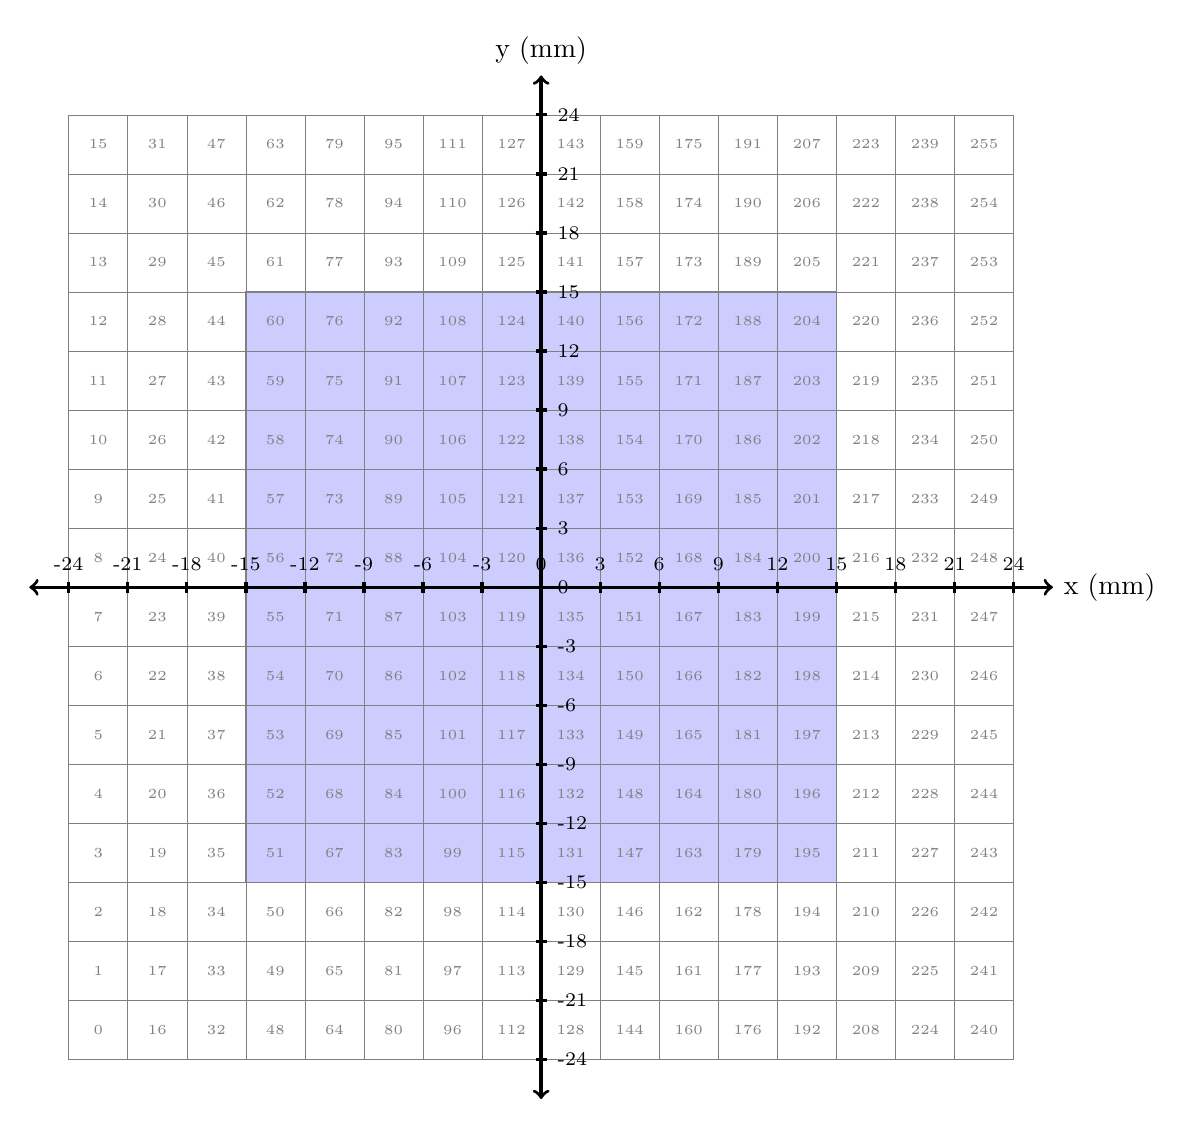
\begin{tikzpicture}
\filldraw[fill=blue!20!white, draw=gray] (-3.75,-3.75) rectangle (3.75,3.75);
\draw[step=0.75cm,gray,very thin] (-6,-6) grid (6,6);
\draw[very thick,<->] (-6.5,0) -- (6.5,0) node[anchor=west] {x (mm)};
\draw[very thick,<->] (0,-6.5) -- (0,6.5) node[anchor=south] {y (mm)};

\foreach \y [count=\yi from 0] in {-5.625,-4.875,...,5.625}
	\foreach \x [count=\xi from 0] in {-5.625,-4.875,...,5.625}
		\pgfmathsetmacro\result{int(round(\yi+16*\xi))}
		\node[gray] at (\x,\y) {\tiny \result};

\foreach \x in {-24,-21,...,24}
	\pgfmathsetmacro\result{\x/4}
	\draw[black,very thick] (\result,-2pt) -- (\result,2pt) node[anchor=south] {\scriptsize \x};
	
\foreach \y in {-24,-21,...,24}
	\pgfmathsetmacro\result{\y/4}
	\draw[black,very thick] (-2pt,\result) -- (2pt,\result) node[anchor=west] {\scriptsize \y};
\end{tikzpicture}

\textit{Figure 1.} 
\end{center} 


\section{Analysis of Data}

The energy deposition was stored in a 1,000,000$\times$256 matrix called \texttt{energy}. The element \texttt{energy$[i][j]$} is the amount of energy deposited in the $j^{th}$ pixel during the $i^{th}$ event. The initial positions of the simulated electrons were stored in a matrix \texttt{position} of size 1,000,000$\times$2. In other words, the initial position for the $i^{th}$ event is given by
\begin{center}
$x_0=$\texttt{position$[i][0]$},\\
$y_0=$\texttt{position$[i][1]$}.
\end{center}



\subsection{Energy Distribution}

For each event $i$, the total energy deposited was calculated by summing over the pixels $j$. A histogram of the total energies is shown below (Figure 2(a)). 

\begin{center}
\begin{figure*}
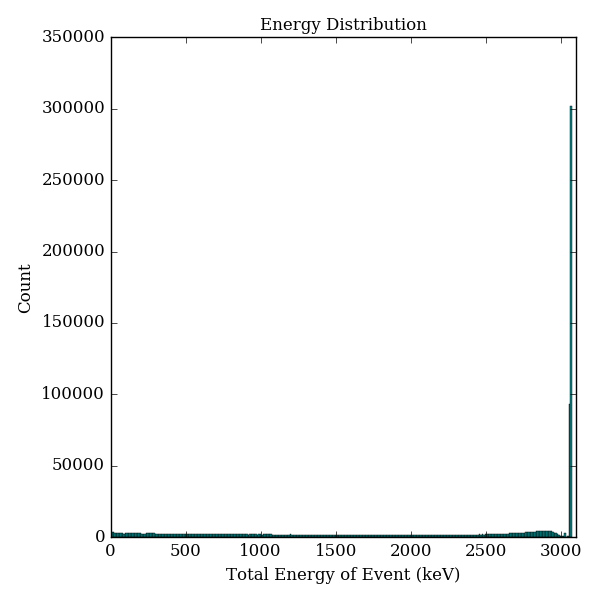
\includegraphics[scale=0.9]{../figures/energy_distribution.png}

\textit{Figure 2(a).} The total energy distribution. There is a clear peak at 3060 keV, the initial energy of the electrons, and a clear dip slightly below the peak. The dip indicates some electrons undergo Brehmsstrahlung radiation and emit a photon with energy $\sim 100$ keV.
\end{figure*}
\begin{figure*}
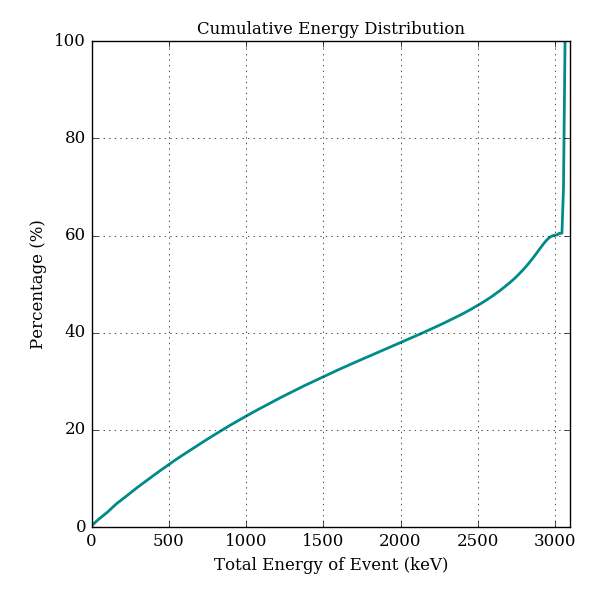
\includegraphics[scale=0.9]{../figures/percentile.png}

\textit{Figure 2(b).} Cumulative energy distribution. The histogram from the previous figure was integrated and normalized. About 60$\%$ of the total energies are below the peak. 
\end{figure*}
\end{center}

\subsection{Correlations}

In the experiment, we will only know how much energy was deposited into each cell (or pixel). One or more cells may be activated in any given event. Using the simulated data, I wanted to learn more about how the initial position $(x_0,y_0)$ of the simulated electron correlated with the cell(s) $\{ j_\alpha, j_\beta, ... \}$ it eventually dumped energy into. The idea is that if cell $j$ was activated, then it's more likely that the electron originated from a position close to or inside cell $j$ than from the other side of the detector. \\


\noindent First, for every cell $j \in [0,255]$ I collected all the initial positions of the electrons which eventually activated cell $j$. This information is stored in corresponding data files named \texttt{cellj.dat}. In figure

\begin{figure*}
\centering
\begin{subfigure}{.5\textwidth}
  \centering
  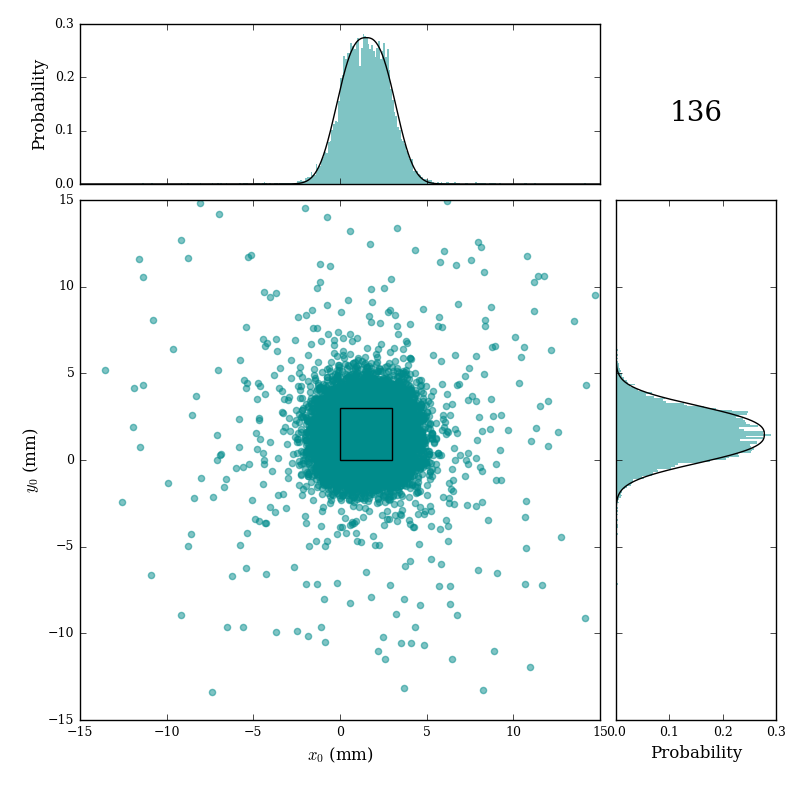
\includegraphics[width=\linewidth]{../figures/cellfigs/cell136.png}
  \label{fig:sub1}
\end{subfigure}%
\begin{subfigure}{.5\textwidth}
  \centering
  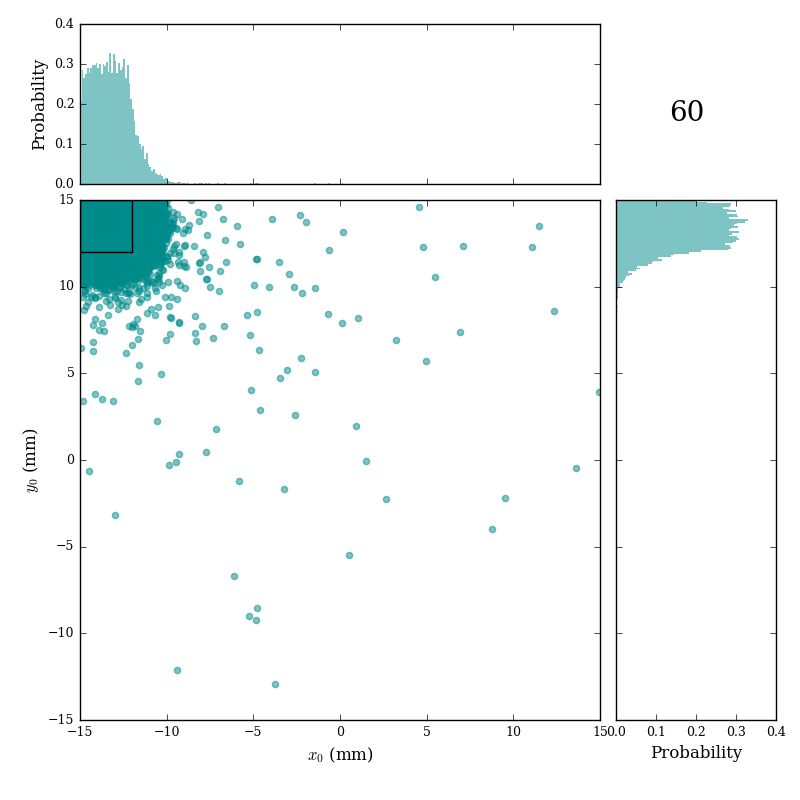
\includegraphics[width=\linewidth]{../figures/cellfigs/cell60.png}
  \label{fig:sub2}
\end{subfigure}
\label{fig:test}

\medskip
\centering
\begin{subfigure}{.5\textwidth}
  \centering
  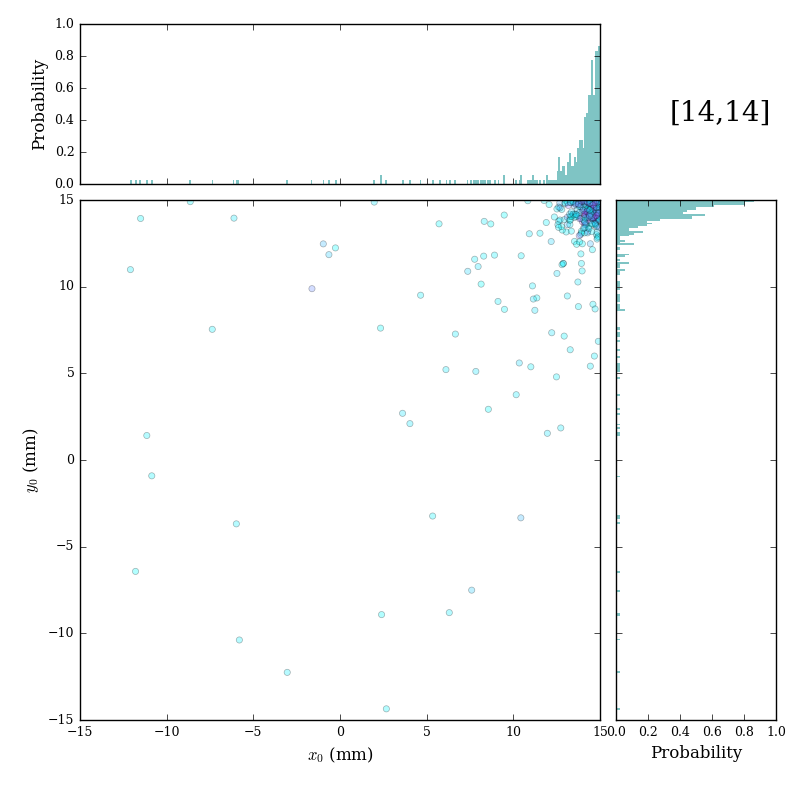
\includegraphics[width=\linewidth]{../figures/cellfigs/cell221.png}
  \label{fig:sub1}
\end{subfigure}%
\begin{subfigure}{.5\textwidth}
  \centering
  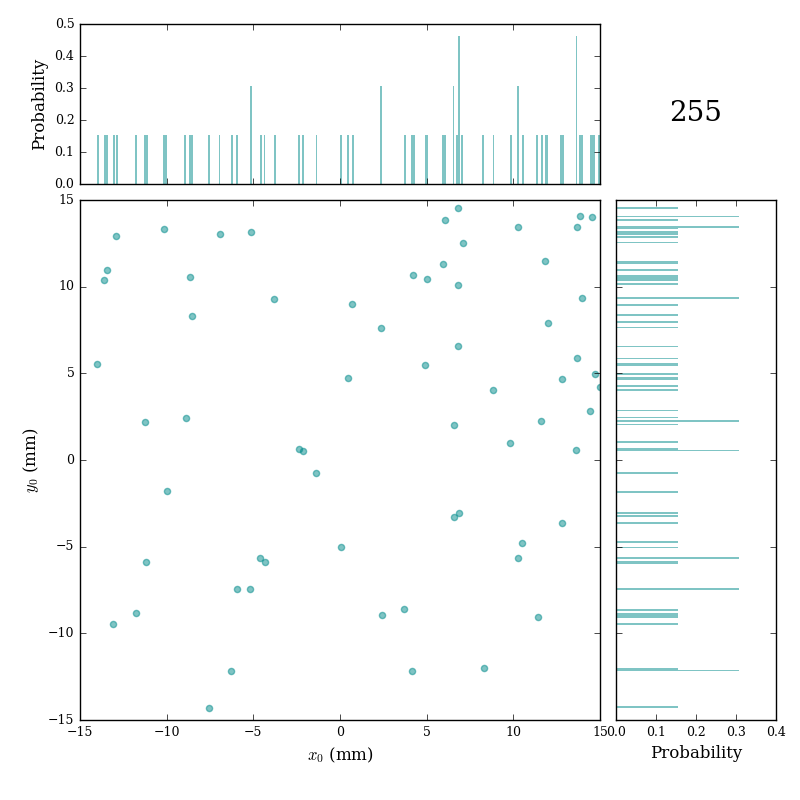
\includegraphics[width=\linewidth]{../figures/cellfigs/cell255.png}
  \label{fig:sub2}
\end{subfigure}
\label{fig:test}
\textit{Figure 3.} Four examples of the distribution of initial positions around a cell. Histograms of the positions in the $x-$ and $y-$directions are given to help understand the shape of the distribution. The histograms were normalized. The black squares in the scatterplots are the outlines of the cells in question.
\end{figure*}

\begin{figure*}
\centering
\begin{subfigure}{.5\textwidth}
  \centering
  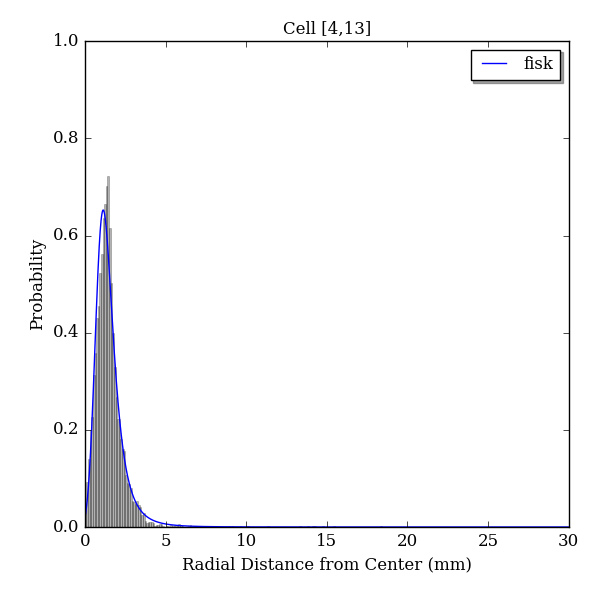
\includegraphics[width=\linewidth]{../figures/cellfigs/probdens60.png}
  \label{fig:sub1}
\end{subfigure}%
\begin{subfigure}{.5\textwidth}
  \centering
  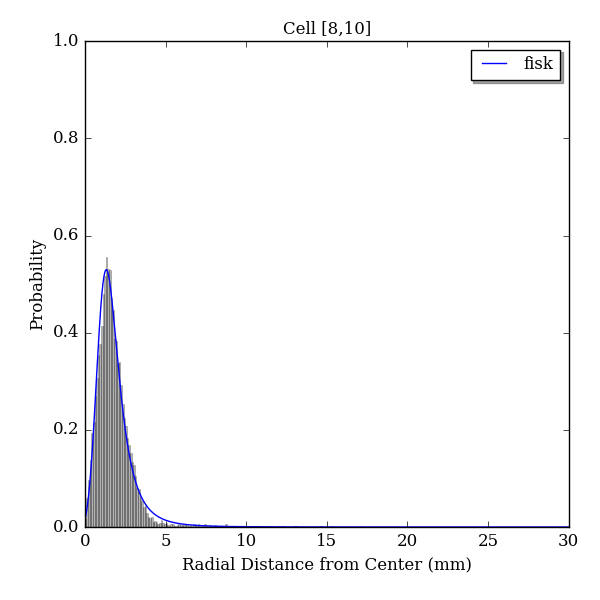
\includegraphics[width=\linewidth]{../figures/cellfigs/probdens121.png}
  \label{fig:sub2}
\end{subfigure}
\label{fig:test}

\medskip
\centering
\begin{subfigure}{.5\textwidth}
  \centering
  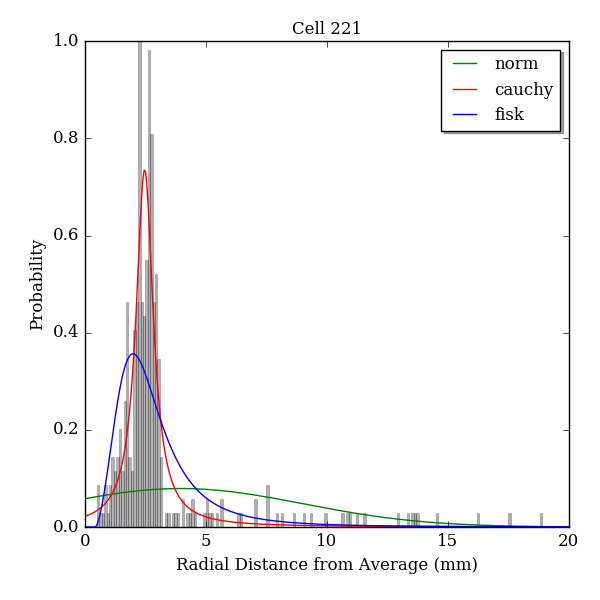
\includegraphics[width=\linewidth]{../figures/cellfigs/probdens221.png}
  \label{fig:sub1}
\end{subfigure}%
\begin{subfigure}{.5\textwidth}
  \centering
  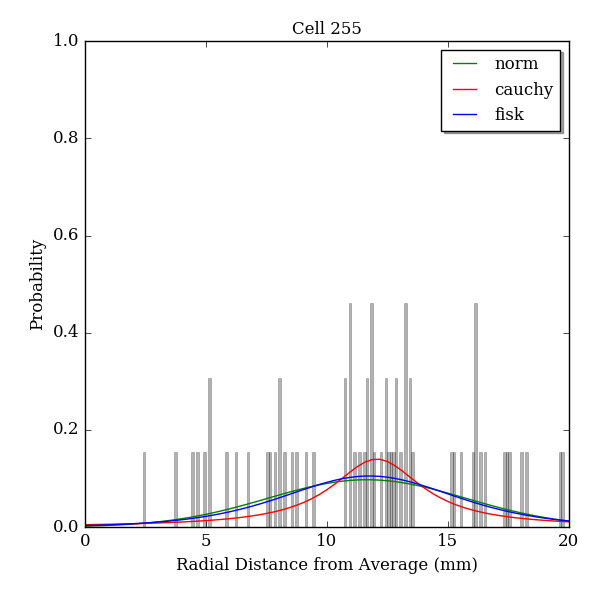
\includegraphics[width=\linewidth]{../figures/cellfigs/probdens255.png}
  \label{fig:sub2}
\end{subfigure}
\label{fig:test}
\textit{Figure 4.} 
\end{figure*}


\begin{center}
\begin{figure*}
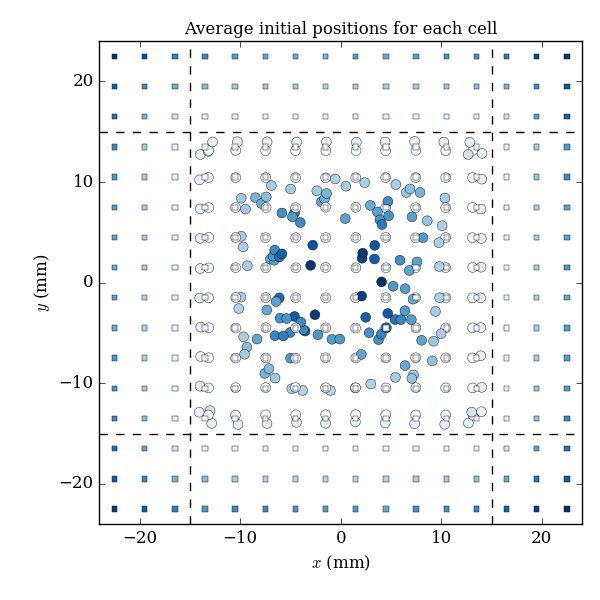
\includegraphics[scale=0.9]{../figures/XY_stats.png}

\textit{Figure 5.} The squares represent the center of each pixel and the circles represent the average initial position of the electrons which hit the pixel. Both squares and circles are colored according to the average distance the electrons travel before hitting the cell.
\end{figure*}
\end{center}





\end{document}
